
\documentclass{article}
\usepackage{amsmath, amssymb, fullpage, dsfont, graphicx, float, verbatim, bm, bbm}

\begin{document}

\title{STA 531: Final Project \\ Predicting Pitches in Baseball}
\author{Sarah Normoyle, Drew Jordan, Gonzalo Bustos}

\maketitle 

\section{Introduction}

Sabermetrics, or the analysis of baseball, has been used widely used by statisticians as a way to analyze the performance of baseball players and baseball teams. The main focus of sabermetrics has been to compare the performance of individual players. There are also other areas of baseball that have been less explored that would be beneficial for players and coaches. The motivation behind this project is that it would greatly valuable for a batter to be to known what pitch to expect before a pitch is thrown. This project is from the outlook of a batter and attempts to be able to predict the following pitch given a sequence of pitches by a pitcher and a set of covariates about the current game play. This information could be used by a batter and a team to be able to predict pitches. 

\section{Data}

This data is found publicly on mlb.com, and we obtained at from a hackathon in Baltimore for the baseball team the Orioles. The data set contains pitching data on all MLB teams over the course of 3 years, from 2013 to 2015. There are 2,114,497 observations of pitches in the data set, and 39 different initial variables. 


\section{Methods}

This project is aimed at applying statistical methods to analyze the pitching sequence of MLB pitchers. Various methods were implemented, and the results were compared to each other. The two main statistical techniques that were used were Markov Models and Multinomial Logistic Regression to predict the sequence of pitches. The sections below go further into detail into the methods used. To be able to compare the different methods, we used cross-validation for each method and used percent accuracy in the predictions as the comparison metric. For each of these methods, we focused on applying the techniques to one particular pitcher.

\subsection{Sampling from Probability Vectors}

The first naive method that was used as a baseline was obtaining the sample probability vectors of throwing the various pitches. This method does not consider any of the covariates. After obtaining a sample probability vector of throwing each pitch, which is obtaining by getting the counts for each pitch and the dividing by the total number of pitches, we can then sample from the different pitch possibilities with probability of the probability vector. Once these predicted pitches are calculated, we obtain the percent accuracy of predictions. We ran this 100 times as there in inherent randomness in the sampling.

\subsection{Markov Model}

Next, a simple Markov model was used. This Markov model only used an initial probability vector and a transition matrix to predict the next pitch in a sequence. The transition matrix was first created from a known set of pitches, and then it can be used to predict the next pitch in a sequence. Cross validation was also applied with this method by training, or creating the transition matrix, on a portion of the data, and then testing this Markov model on the held out set. The percent accuracy in predictions was once again used as the comparison metric.  

\subsection{Hidden Markov Model}

After applying a simple Markov model, a more complex hidden Markov model was implemented to the pitching sequences. Given a sequence of pitches, to obtain the optimal parameters for the model, the Baum-Welch algorithm was used. Once these parameters were determined, to obtain the probabilities of the following observation given the previous observations, $p(x_{n+1} | x_{1:n})$, the Forward Algorithm was then implemented. Both algorithms are described more in detail below.

\subsubsection{Baum-Welch}

The Baum-Welch algorithm applies expectation maximization to hidden Markov models to obtain parameters for the Hidden Markov Model, which are the inital probability vector, the transition matrix from state to state, and the emission matrix. The Baum-Welch algorithm is an iterative algorithm that uses the forward-backward algorithm at each iteration to estimate these parameters.  \\ 
\\ 
The forward-backward algorithm is as follows: \\
\\ 
In the forward algorithm, we sum over $z_1, z_2, \hdots, z_n$ in that order, and derive a recursion for computing $p(x_{1:j}, z_j)$ for each $z_j = 1,\hdots,m$ and each $j = 1,\hdots,n$. In the backward algorithm, we sum over $z_n, z_{n-1}, \hdots, z_1$, and derive a recursion for computing $p(x_{j+1:n} | z_j)$ for each $z_j = 1,\hdots,m$ and each $j = 1,\hdots,n$. \\ 
\\ 
The forward-backward algorithm was implemented as shown below. The log of the probabilities were taken in order to deal with arithmetic underflow/overflow and R's inability to store such a low probability. In addition, the log-sum-exp trick was used to deal with a similar problem. \\
\\
Forward algorithm: \\ 
1. For each $z_1,\hdots, m,$ compute $g_1(z_1) = \log p(z_1) + \log p(x_1 | z_1)$ \\ 
2. For each $j = 2, \hdots, n$ for each $z_j = 1,\hdots, m,$ compute:
$$\log s_j(z_j) = g_j(z_j) = \log \sum_{z_{j-1}} \exp [g_{j-1}(z_{j-1}) + \log p(z_j | z_{j-1}) + \log p(x_j|z_j) ] $$
3. $\log p(x_{1:n}) = \log \sum_{z_n} \exp(g_n(z_n))$ \\ 
\\
And $g_j(z_j) = \log p(x_{1:j}, z_j)$ \\
\\ 
Backward algorithm: \\ 
1. For each $z_n = 1,\hdots, m,$ define $r_n(z_n) = 0$ \\ 
2. For each $j = n - 1, n - 2, \hdots, 1,$ for each $z_j = 1,\hdots,m$ compute:
$$r_j(z_j) = \log \sum_{z_{j+1}} \exp (\log p(z_{j+1}|z_j) + \log p(x_{j+1}|z_{j+1}) + r_{j+1} (z_{j+1}))$$ \\ 
\\ 
And $r_j(z_j) = \log p(x_{j+1:n}|z_j)$ \\ 
\\ 
The Baum-Welch algorithm is implemented as follows:
\\ 
Using the following formula: \\
$$\gamma_{ti} = P(Z_t = i|x) $$
$$\beta_{tij} = P(Z_{t-1} = i, Z_t = j |x) $$
$$\pi_j = \dfrac{\gamma_{1i}}{\sum_{j=1}^m \gamma_{1j}}$$
$$T_{ij} = \dfrac{\sum_{t=2}^n \beta_{tij}}{ \sum_{t=1}^{n-1} \gamma_{ti}}$$ 
\\ 
The algorithm is: \\ 
1. Randomly initialize $\pi, T, $ and $\phi = (\phi_1,\hdots, \phi_m)$\\ 
2. Iteratively repeat the following two steps, until convergence: \\ 
(a) E-step: Compute the $\gamma$ and $\beta$ using the forward-backward algorithm.\\ 
(b) M-step: Update $\pi, T,$ and $\phi$ using the formulas above.\\
\\ 
This algorithm was implemented in Python, and the results from the Baum-Welch were used in the Forward algorithm to do probabilistic inference, which is described below. 

\subsubsection{Forward Algorithm}

Once the parameters are estimated for the transition matrix, the emission matrix, and the initial probability matrix, we can combine these parameters with results from the forward algorithm to get probabilities for the next observation given the previous observation.  \\ 
\\ 
We can predict $x_{j+1}$ and $x_{1:j}$ using: \\ 
$$p(x_{j+1}|x_{1:j}) \propto p(x_{1:j}, x_{j+1}) = \sum_{z_j, z_{j+1}} p(x_{1:j}, x_{j+1}, z_j, z_{j+1})$$
$$ = \sum_{z_j, z_j+1} p(x_{1:j}, z_j) p(z_{j+1}|z_j) p(x_{j+1}|z_{j+1})$$
\\ 
Cross validation was also applied in this setting. The Baum-Welch algorithm was applied to the training set. Then as we ran through a sequence of observations in the testing set, we can use the forward algorithm and the estimate parameters to get probabilities of the next observation. These predictions are compared to the true predictions in order to obtain an estimated percent accuracy in predictions.

\subsection{Multinomial Logistic Regression}

After Markov models were implemented, multinomial logistic regression models were then fit to predict the pitch given a set of covariates. Multinomial logistic regression is a classification scheme that generalizes logistic regression to a multivariate scheme. Because a pitcher can throw multiple types of pitches at a given observation, we have a vector of possible pitches. \\
\\ 
Given the multinomial data with J categories and the p-dimensional predictor variables, we can forecast in which j category a future data point $y^*$ at the predictor $x^*$ will be. \\
\\
Multinomial logistic regression can be understood as a set of independent binary regressions. If we have J possible outcomes, we can imagine running $J-1$ binary regression regression models, which are compared against the one pivot outcome. 

$$ \frac{\Pr(Y_i=1)}{\Pr(Y_i=K)} = \beta_1 \cdot {X}_i $$
$$ \frac{\Pr(Y_i=2)}{\Pr(Y_i=K)} = \beta_2 \cdot {X}_i $$
$$ \cdots \cdots$$ 
$$ \frac{\Pr(Y_i=K-1)}{\Pr(Y_i=K)} = \beta_{K-1} \cdot {X}_i$$ 

\noindent For each possible outcome, there are separate vectors of regression coefficients. Therefore, we can calculate the probability of observing a category j after at a time occurrence as: 

$$ P(y^* = j | x^*, \beta, n^* = 1 ) = e^{x^* \beta_j} / \sum_{k=1}^{J} e^{x^* \beta_k}. $$

\noindent Once we calculate these probabilities for a set of covariates, we can predict what the pitch will be for the set of covariates.  \\ 
\\ 
For this dataset, there were specific variables that were intended to be used in the model, as they have known to make a difference in pitching. There were also some attempts at variable selection by choosing variables that created the highest percent accuracy when implemented on the testing set. 

\subsection{Cross Validation}

5-fold Cross Validation was also implemented for the various methods. Cross validation is a model validation technique to assess how statistical analysis will generalize to another independent data set. In cross validation, we divide the dataset into a training set and a test set. The training set's covariates and pitches are used to run and train the model, and the covariates of the test set are used to predict the pitches. The predicted pitches are then compared to the true pitches in the test set. The 5 folds refers to the number of times we divide the data into training and test sets. We average the results across the 5 different results. Cross validation is helps problems such as over-fitting a dataset because it tests the model against another dataset. 

\section{Results}

\subsection{Exploratory Data Analysis}

First, some exploratory data analysis was conducted to get a feel for the data and see if certain covariates varied across the different types of pitches. Below are some of the results from the exploratory data analysis.


\subsection{Predicting and Cross Validation}

The various methods descried in the Methods section were implemented for the pitcher Clayton Kershaw. He only pitches four different type of pitches, and he has numerous pitch observations in the dataset. These methods include sampling from the sample probability vector, a simple Markov chain, a hidden Markov model, and various multinomial logistic regression models. The total percent accuracy was calculated for each method. The only issue came with implementing the Baum-Welch algorithm. After many attempts, the product of the algorithm did not produce viable results, and therefore, the results are not included below. For the logistic regression, a simple variable selection process was done for looking to add variables that would allow the model to have the highest percent accuracy. The variable ``count'' (as is balls, strikes) was found to make the biggest difference in percent accuracy followed by ``inning'' and ``previous pitch''. After those variables, adding or changing other variables did not make much of a difference. Therefore, we have shown results for three models with the following variables used:\\ 
\begin{center}
\begin{tabular}{|l|l|}
	\hline
	Model \# & Variables \\ 
	\hline
	LR1  & count \\ 
	\hline
	LR2  & count, pre outs, inning \\
	\hline
	LR3  & pre outs, count, pitch number, runners count, pitch count \\ 
	& top inning, bat side, inning, prev pitch type \\
	\hline
\end{tabular}
\end{center}

\noindent The results of these from testing within sample is shown below.

% latex table generated in R 3.2.2 by xtable 1.7-4 package
% Thu May  5 18:03:12 2016
\begin{table}[ht]
\centering
\begin{tabular}{rrrrrr}
  \hline
 & CH & CU & FF & SL & Total \\ 
  \hline
Sampling & 0.0231 & 0.1337 & 0.5715 & 0.2700 & 0.4180 \\ 
  Markov & 0.0154 & 0.1691 & 0.5742 & 0.2666 & 0.4208 \\ 
  LR1 & 0.0000 & 0.2770 & 0.8886 & 0.1178 & 0.5795 \\ 
  LR2 & 0.0000 & 0.2349 & 0.9074 & 0.1132 & 0.5827 \\ 
  LR3 & 0.0000 & 0.3301 & 0.8855 & 0.1283 & 0.5885 \\ 
   \hline
\end{tabular}
\caption{Percent Accuracies from In-Sample Testing} 
\end{table}


\noindent The results from testing using 5-fold Cross Validation is shown below.

% latex table generated in R 3.2.2 by xtable 1.7-4 package
% Thu May  5 18:02:51 2016
\begin{table}[ht]
\centering
\begin{tabular}{rrrrrr}
  \hline
 & CH & CU & FF & SL & Total \\ 
  \hline
Sampling & 0.0000 & 0.1484 & 0.5719 & 0.2665 & 0.4183 \\ 
  Markov & 0.0515 & 0.1420 & 0.5647 & 0.2616 & 0.4188 \\ 
  LR1 & 0.0140 & 0.2884 & 0.6392 & 0.2972 & 0.4873 \\ 
  LR2 & 0.0444 & 0.3029 & 0.6342 & 0.3062 & 0.4902 \\ 
  LR3 & 0.0478 & 0.2893 & 0.6347 & 0.3159 & 0.4949 \\ 
   \hline
\end{tabular}
\caption{Percent Accuracies from Cross Validation} 
\end{table}


\noindent These tables shown below as bar plots.

\begin{center}
		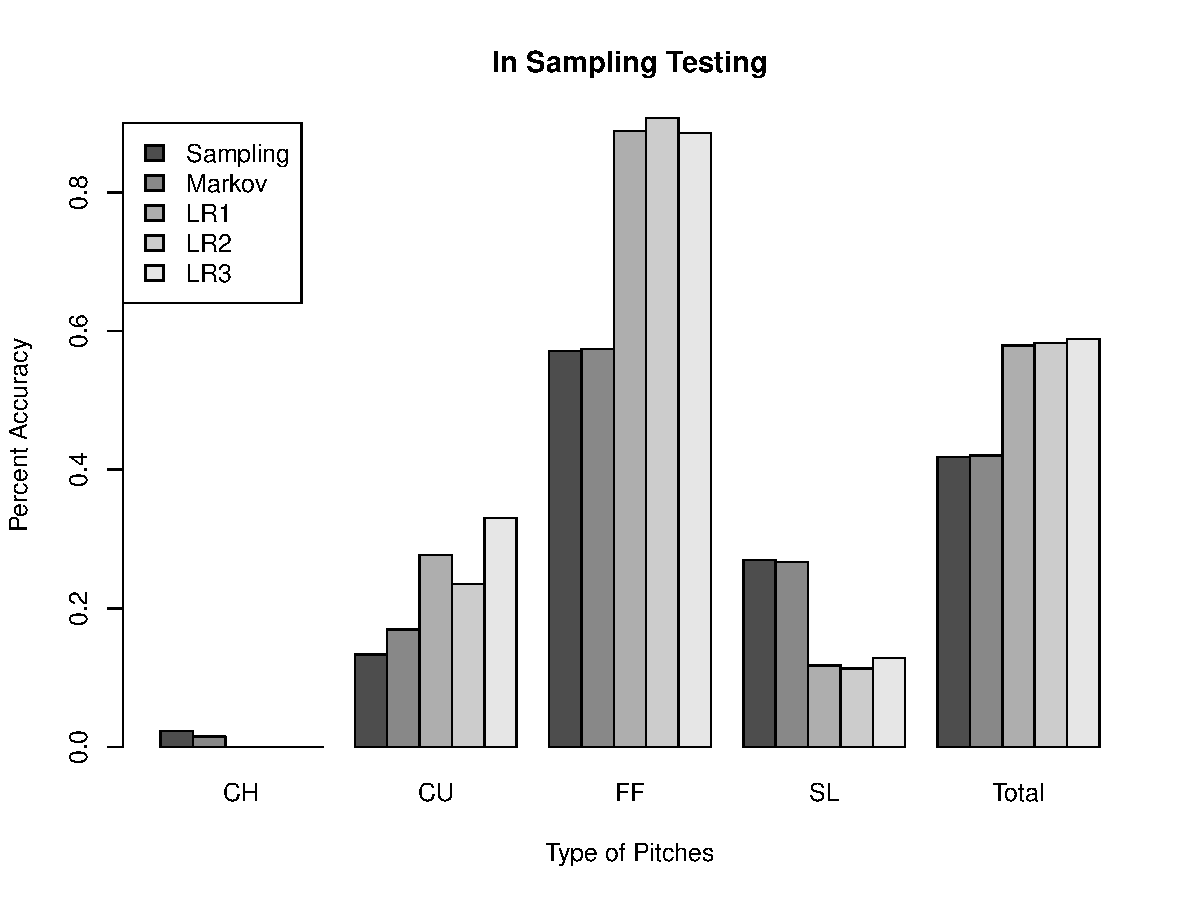
\includegraphics[scale = .7]{NOT_CV.pdf}
\end{center}

\begin{center}
		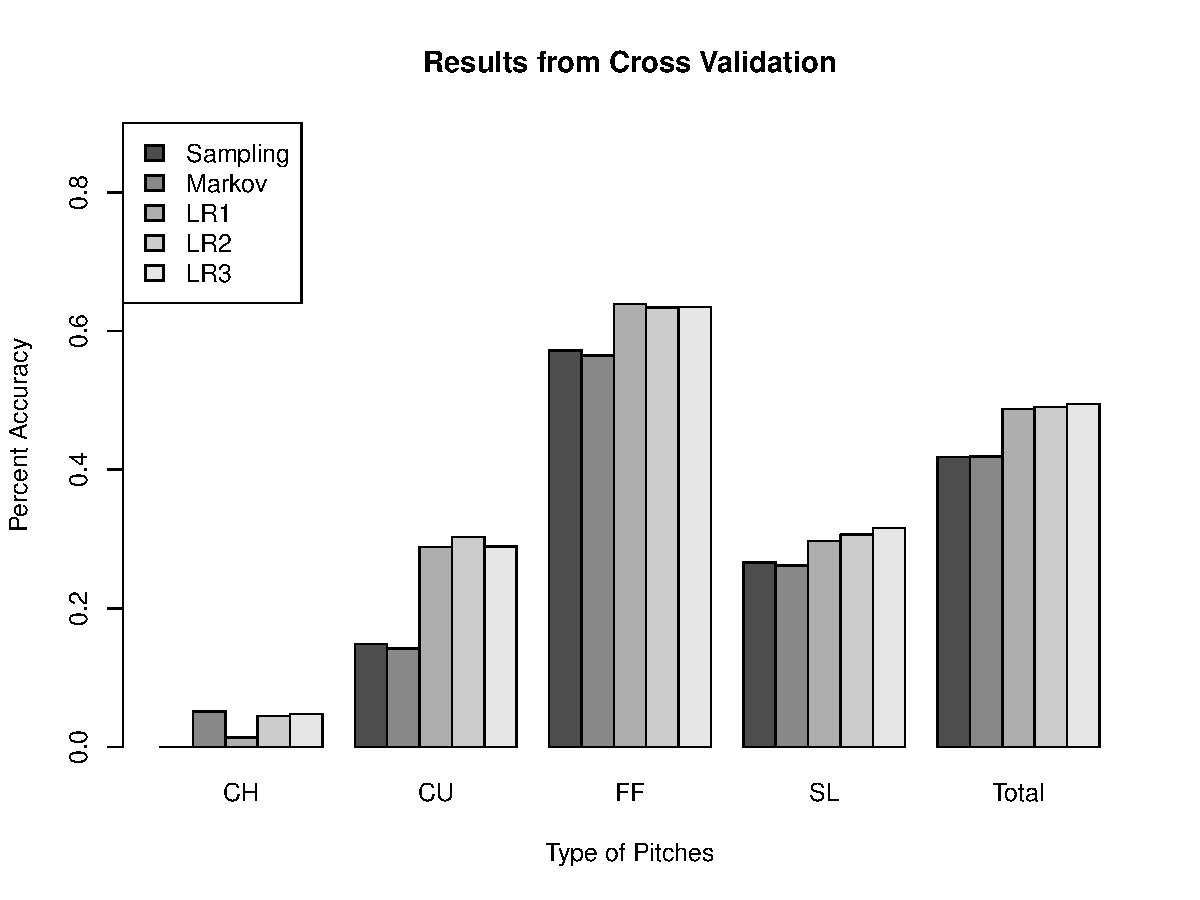
\includegraphics[scale = .7]{CV.pdf}
\end{center}

\noindent As we can see from the tables and the bar plots, the best performing models are the multinomial logistic regression models. The Markov model does not have a much better performance than simply sampling from the probability vector. We can also see that predicting fast balls seems to be more accurate than other pitches. The cross validation technique also shows that it is a necessary technique to be able to accurately show the results of a model rather than simply doing in sample testing. 

\section{Conclusion}

After applying different statistical methods, there has been shown some results in ability to predict baseball pitches. The applications of various Markov models and multinomial logistic regression has also been shown to be useful as well as the success of cross validation to check the results of a model. However, there is still much room for improvement in predicting baseball pitches. This project focused on the pitches of one particular pitcher because of various pitch styles and complications with adding in multiple pitchers. This project can be further investigating by examining multiple pitchers and the differences in predicting pitches by different pitchers. 




\end{document}